\documentclass[paper=a4, fontsize=11pt]{scrartcl}
\usepackage[T1]{fontenc}
\usepackage{fourier}

\usepackage[english]{babel}															% English language/hyphenation
\usepackage[protrusion=true,expansion=true]{microtype}	
\usepackage{amsmath,amsfonts,amsthm} % Math packages
\usepackage[pdftex]{graphicx}	
\usepackage{url}
\usepackage{hyperref}


%%% Custom sectioning
\usepackage{sectsty}
\allsectionsfont{\centering \normalfont\scshape}
\usepackage{subfigure}
\usepackage{comment}


%%% Custom headers/footers (fancyhdr package)
\usepackage{fancyhdr}
\pagestyle{fancyplain}
\fancyhead{}											% No page header
\fancyfoot[L]{}											% Empty 
\fancyfoot[C]{}											% Empty
\fancyfoot[R]{\thepage}									% Pagenumbering
\renewcommand{\headrulewidth}{0pt}			% Remove header underlines
\renewcommand{\footrulewidth}{0pt}				% Remove footer underlines
\setlength{\headheight}{13.6pt}


%%% Equation and float numbering
%\numberwithin{equation}{section}		% Equationnumbering: section.eq#
%\numberwithin{figure}{section}			% Figurenumbering: section.fig#
%\numberwithin{table}{section}				% Tablenumbering: section.tab#


%%% Maketitle metadata
\newcommand{\horrule}[1]{\rule{\linewidth}{#1}} 	% Horizontal rule

\title{
		%\vspace{-1in} 	
		\usefont{OT1}{bch}{b}{n}
		\normalfont \normalsize \textsc{CS650 - Computer Vision} \\ [25pt]
		\horrule{0.5pt} \\[0.4cm]
		\huge Programming Lab 5 \\ Image Stitching \\
		\horrule{2pt} \\[0.5cm]
}
\author{
		\normalfont %\normalsize
        Tim Price \and Daqing Yi \\
}
%\date{}


%%% Begin document
\begin{document}
\maketitle

\begin{comment}
Step 1: Calculate Homography 
 high-contrast corners (Manual)
Step 2: Warp images
 backward mapping method (bilinear interpolation)
 
Extra credits:
(1) stitch the images by using a simple blending of them
(2) Use linear regression (more than four points)
(3) Use RANSAC (support bad point matches)
(4) Find points automatically using point detectors
\end{comment}

\begin{comment}
(1) GUI
Create GUI framework (DQ)
File loading (Tim)
Image displaying (DQ)
(2) Homography
Four point algorithm
(3) Warp
(3.1)Display a warped polygon
(3.2)Fill pixels using billinear interpolation
(4) Blending
(4.1) Average
(4.2) Weighted average
(5) Linear Regression
(6) RANSAC
\end{comment}

\section{Introduction}
%Tim

\section{Computing Homography}
%DQ

Homography is used to denote the transformation from one image plane to the other.
It is written as 
\begin{equation}
\label{eq:homography}
\begin{bmatrix}
x' \\
y' \\
1
\end{bmatrix}
\sim
\begin{bmatrix}
\tilde{x}' \\
\tilde{y}' \\
\tilde{w}'
\end{bmatrix}
=
\begin{bmatrix}
h_{00} & h_{01} & h_{02} \\
h_{10} & h_{11} & h_{12} \\
h_{20} & h_{21} & 1 
\end{bmatrix}
\begin{bmatrix}
x \\
y \\
1
\end{bmatrix}
\end{equation}
By writing Equation \ref{eq:homography} as
\begin{equation}
\begin{bmatrix}
x & y & 1 & 0 & 0 & 0 & -x'x & -x'y \\
0 & 0 & 0 & x & y & 1 & -y'x & -y'y
\end{bmatrix}
\begin{bmatrix}
h_{00} \\
h_{01} \\
h_{02} \\
h_{10} \\
h_{11} \\
h_{12} \\
h_{20} \\
h_{21} 
\end{bmatrix}
=
\begin{bmatrix}
x' \\ y'
\end{bmatrix},
\end{equation}
having four points (no three points in a line) is enough to calculate the homography. 
The implementation is in \emph{calcHomograph} method in \emph{ImageManager.py}.
In order to verify the correctness of the homography, the points are mapped into same image plane and the differences are compared.



\section{Warping the Images}
%Tim
\begin{figure}[h]
\centering
\subfigure[Warp \emph{IMG\_1343.JPG} to the image plane of \emph{IMG\_1341.JPG}.]{
\includegraphics[width=.45\textwidth]{./figure/2_to_0.png} 
\label{fig:warping:01} } 
\subfigure[Warp \emph{IMG\_1345.JPG} to the image plane of \emph{IMG\_1341.JPG}.]{
\includegraphics[width=.45\textwidth]{./figure/4_to_0.png} 
\label{fig:warping:02} } 
\caption{Image warping.}
\label{fig:warping}
\end{figure}

\section{Extra}

\subsection{Stitching the images}
%Tim

\begin{figure}[h]
\centering
\subfigure[Blend \emph{IMG\_1342.JPG} with \emph{IMG\_1341.JPG}.]{
\includegraphics[width=.45\textwidth]{./figure/1_and_0.png} 
\label{fig:blending:01} } 
\subfigure[Blend \emph{IMG\_1344.JPG} with \emph{IMG\_1341.JPG}.]{
\includegraphics[width=.45\textwidth]{./figure/3_and_0.png} 
\label{fig:blending:02} } 
\caption{Image blending.}
\label{fig:blending}
\end{figure}

\begin{figure}[h]
\centering
\includegraphics[width=\textwidth]{./figure/1_2_3_4_and_0.png} 
\caption{Stitched image.}
\label{fig:stitched_image}
\end{figure}

\subsection{Homograph Calculation using linear least squares}
%DQ

\subsection{RANSAC}
%Tim

\subsection{Automatic point detection}
%DQ

\subsubsection{Harris corner detector}

\begin{figure}[h]
\centering
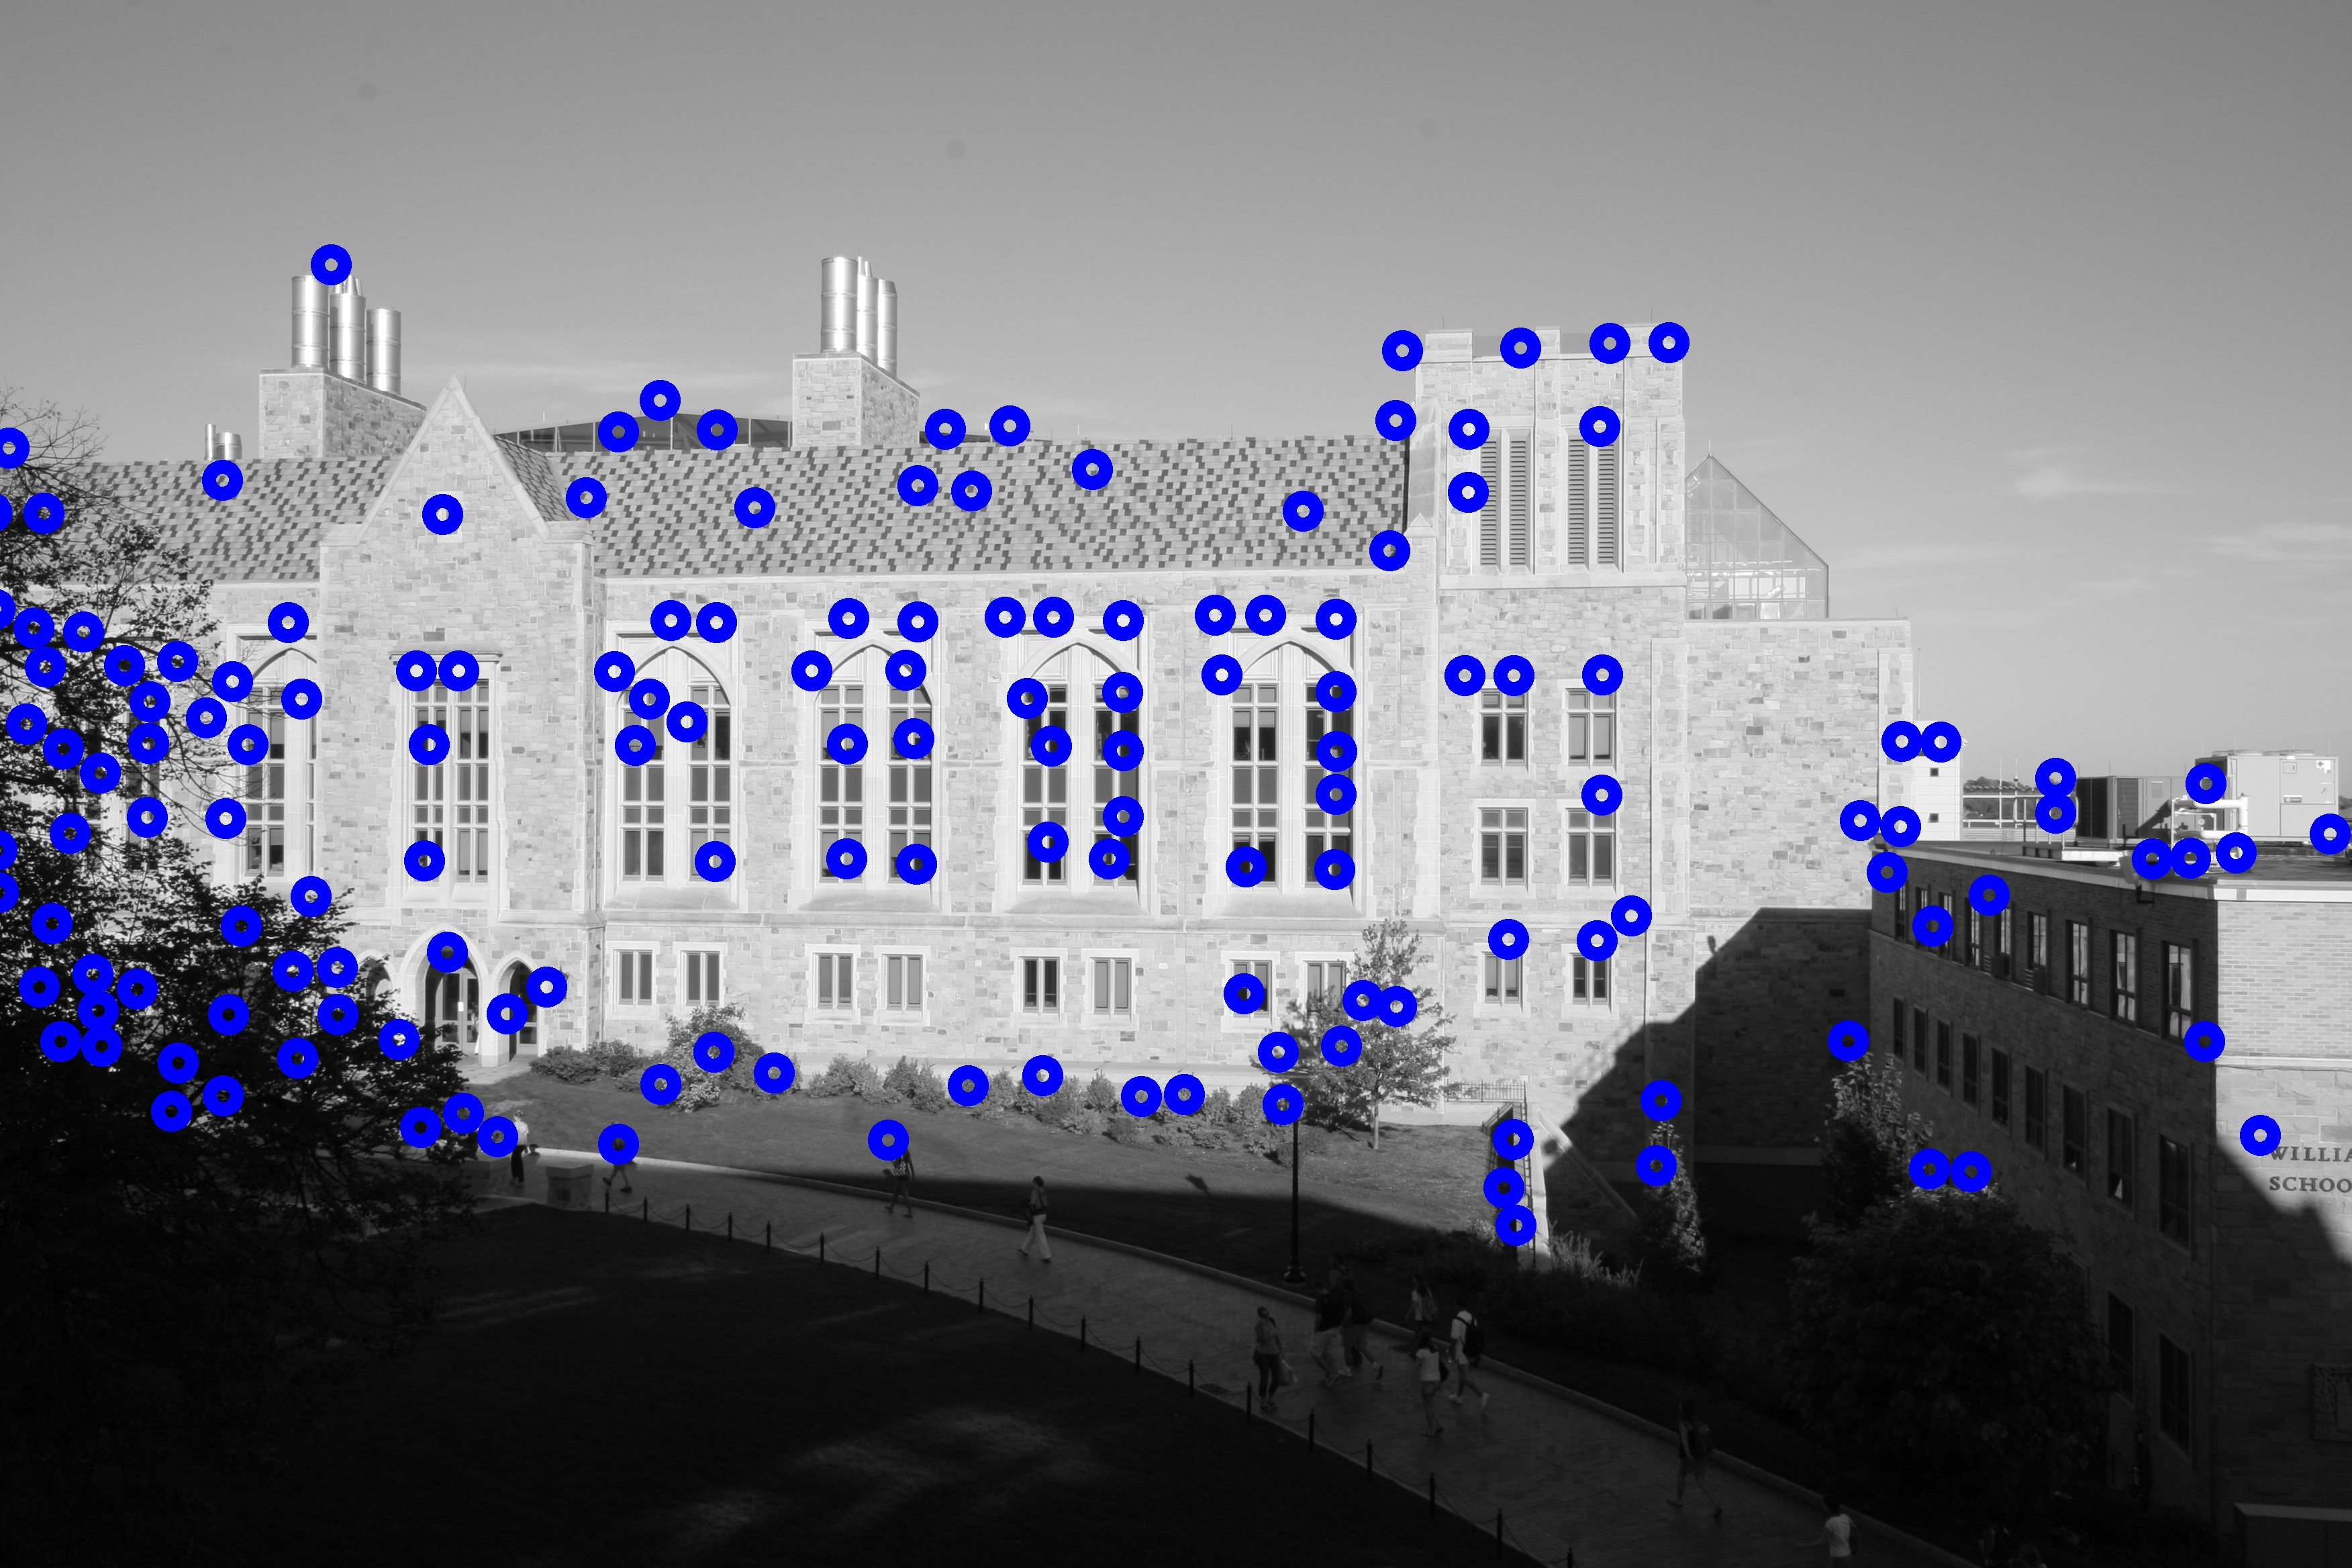
\includegraphics[width=.8\textwidth]{./figure/IMG_1341_hcd.jpg} 
\caption{Apply Harris corner detector to \emph{IMG\_1341.JPG}.}
\label{fig:corner_detection}
\end{figure}

\subsubsection{Prematch - Normalized Cross-Correlation}

\textbf{Normalized Cross-Correlationn} is used to measure the similarities of two points when doing prematch.
It is defined as 
\begin{equation}
\mbox{ncc} = \frac{1}{n} \sum_{x, y} \frac{(I_{1}(x,y)-\bar{I}_{1})(I_{2}(x,y)-\bar{I}_{2})}{\sigma_{1}\sigma_{2}}
\end{equation}



\subsubsection{Applying RANSAC}



\section{Conclusion}






\bibliography{reference}
\bibliographystyle{plain}

\end{document}